\documentclass{article}
\usepackage[utf8]{inputenc}
\usepackage{CJKutf8}
\usepackage{graphicx}
\usepackage{subfig}
\usepackage{float}

\usepackage{tikz}
\usepackage{xcolor}

% Custom colors
\definecolor{process0}{RGB}{144,202,249}  % Light blue
\definecolor{process1}{RGB}{165,214,167}  % Light green
\definecolor{process2}{RGB}{255,204,128}  % Light orange
\definecolor{process3}{RGB}{206,147,216}  % Light purple
\definecolor{halocell}{RGB}{239,154,154}  % Light red

\usepackage{dirtree}

% Layout
\usepackage[left=1.5in, right=1.5in, top=1in, bottom=1in]{geometry}

% Images
\graphicspath{{./images/}}
\usepackage{wrapfig}
\usepackage{tabularx}
\usepackage{multirow}
\usepackage{totalcount}
\usepackage{caption}
\captionsetup{skip=0pt} 




% Math
\usepackage{amsmath,amssymb,amsthm,enumitem,bm}

\DeclareMathOperator{\sech}{sech}
\DeclareMathOperator{\csch}{csch}
\DeclareMathOperator{\arcsec}{arcsec}
\DeclareMathOperator{\arccot}{arcCot}
\DeclareMathOperator{\arccsc}{arcCsc}
\DeclareMathOperator{\arccosh}{arcCosh}
\DeclareMathOperator{\arcsinh}{arcsinh}
\DeclareMathOperator{\arctanh}{arctanh}
\DeclareMathOperator{\arcsech}{arcsech}
\DeclareMathOperator{\arccsch}{arcCsch}
\DeclareMathOperator{\arccoth}{arcCoth}

\usepackage{listings}
\usepackage{parskip}
\setlength{\parindent}{0pt}

\begin{document}
% Title
\begin{center}
    \huge\textbf{M2: Lora Finetuning}
\end{center}



\begin{center}
    \Large Xueqing Xu (xx823)
    
    Department of Physics, University of Cambridge
    
    April 7, 2025
\end{center}

\section*{Introduction}
We fine-tune the Qwen2.5-Instruct LLM for predator-prey population forecasting using Low-Rank Adaptation (LoRA). While LLMs can perform time series forecasting without explicit training\cite{gruver2023large}, we investigate how targeted fine-tuning enhances these capabilities under computational constraints.

LoRA injects trainable low-rank matrices into existing weights without modifying original parameters, dramatically reducing trainable parameter count. This parameter-efficient approach is ideal for large models under limited compute budgets.
\section*{Methodology}
\subsection*{Qwen2.5-Instruct model architecture}
The Qwen2.5-0.5B-Instruct model implements a decoder-only transformer architecture with 494 million parameters (Table \ref{tab:qwen25-overview}). With a hidden dimension of 896 across 24 transformer layers, the model balances depth and computational efficiency.

A key architectural feature is Grouped Query Attention (GQA), which employs 14 query heads but only 2 key-value heads—a 7:1 ratio that substantially reduces memory usage during inference while maintaining attention capabilities. For normalization, Qwen2.5 uses RMSNorm with $\epsilon = 10^{-6}$, which offers better training stability than traditional LayerNorm.

% Qwen2.5-0.5B-Instruct Model Overview Table
\begin{table}[ht]
\centering
\begin{tabular}{ll}
\hline
\textbf{Parameter} & \textbf{Value} \\
\hline
Model Type & Decoder-only Transformer \\
Parameters & 0.5 Billion \\
Hidden Size & 896 \\
Attention Heads & 14 \\
Head Dimension & 64 \\
Number of Layers & 24 \\
Intermediate Size (MLP) & 4864 \\
Vocabulary Size & 151,936 \\
\hline
\multicolumn{2}{l}{\textbf{Layer Structure (Repeated 24 times):}} \\
\hline
Pre-Attention & RMSNorm \\
Attention & Multi-head attention with RoPE \\
& \quad - Q, K, V projections \\
& \quad - Rotary Position Embeddings \\
Post-Attention & Residual connection \\
Pre-MLP & RMSNorm \\
MLP & Gate and Up projections \\
& SwiGLU activation \\
& Down projection \\
Post-MLP & Residual connection \\
\hline
\textbf{Final Output} & RMSNorm + Linear (LM head) \\
\hline
\end{tabular}
\caption{Qwen2.5-0.5B Model Architecture}
\label{tab:qwen25-overview} 
\end{table}

\subsubsection*{Key Components with Mathematical Definitions}

\textbf{RMSNorm (Root Mean Square Normalization):} Unlike traditional LayerNorm, RMSNorm eliminates mean-centering and focuses only on variance normalization:

\begin{equation}
\text{RMSNorm}(x) = \frac{x}{\sqrt{\frac{1}{n}\sum_{i=1}^{n}x_i^2 + \epsilon}} \cdot \gamma
\end{equation}

\noindent where $\epsilon = 10^{-6}$ is a small constant for numerical stability, and $\gamma$ represents trainable scale parameters.

\textbf{SiLU (Swish) Activation:} The SiLU activation function used in the feed-forward networks is defined as:
\begin{equation}
\text{SiLU}(x) = x \cdot \sigma(x) = \frac{x}{1 + e^{-x}}
\end{equation}

\noindent where $\sigma(x)$ is the sigmoid function. This activation combines properties of both ReLU and sigmoid functions.

\textbf{Rotary Position Embeddings (RoPE):} RoPE\cite{su2024roformer} encodes position information through rotation matrices in the complex plane:

\begin{equation}
\mathbf{q}_{m,i}^{\theta} = \begin{pmatrix} \cos(m\theta_i) & -\sin(m\theta_i) \\ \sin(m\theta_i) & \cos(m\theta_i) \end{pmatrix} \mathbf{q}_{m,i}
\end{equation}

\noindent where $\mathbf{q}_{m,i}$ represents query vector components, $m$ is the position index, and $\theta_i$ denotes frequencies constructed with base $\theta = 1,000,000.0$.

\textbf{SwiGLU Feed-Forward Network:} The FFN in each layer consists of three projections:

\begin{enumerate}
\item \textbf{Gate Projection:} $G(x) = W_g x$, where $W_g \in \mathbb{R}^{4864 \times 896}$
\item \textbf{Up Projection:} $U(x) = W_u x$, where $W_u \in \mathbb{R}^{4864 \times 896}$
\item \textbf{Down Projection:} $D(x) = W_d x$, where $W_d \in \mathbb{R}^{896 \times 4864}$
\end{enumerate}

The complete FFN operation is defined as:
\begin{equation}
\text{FFN}(x) = D(\text{SiLU}(G(x)) \odot U(x))
\end{equation}

\noindent where $\odot$ represents element-wise multiplication.

% Qwen2.5-0.5B-Instruct Vocabulary Details Table
\begin{table}[H]
\centering
\begin{tabular}{@{}ll@{}}
\hline
\textbf{Property} & \textbf{Value} \\
\hline
Vocabulary Size & 151,936 tokens \\
BOS Token ID & 151,643 \\
EOS Token ID & 151,645 \\
Word Embeddings & Tied with output layer \\
\hline
\end{tabular}
\caption{Qwen2.5-0.5B-Instruct Vocabulary Details}
\label{tab:qwen25-vocab}
\end{table}

The model implements these components with a vocabulary of 151,936 tokens and tied word embeddings between input and output layers (Table \ref{tab:qwen25-vocab}). This architecture is particularly suitable for parameter-efficient fine-tuning methods like LoRA, as we can target high-leverage components (query and value projections) while keeping most parameters frozen.
\subsection*{Lora Finetuning}
Low-Rank Adaptation (LoRA) \cite{hu2022lora} represents a parameter-efficient fine-tuning approach that substantially reduces the number of trainable parameters while maintaining model performance. The key innovation lies in decomposing weight updates into low-rank matrices instead of fine-tuning the entire weight matrices.

\subsubsection*{Mathematical Formulation}

In standard fine-tuning of a pre-trained model, the weight matrix $W_0 \in \mathbb{R}^{d \times k}$ is updated to $W = W_0 + \Delta W$ during training. LoRA parameterizes the update $\Delta W$ using two low-rank matrices:

\begin{equation}
W = W_0 + \Delta W = W_0 + BA
\end{equation}

where $B \in \mathbb{R}^{d \times r}$ and $A \in \mathbb{R}^{r \times k}$ with rank $r \ll \min(d,k)$. During the forward pass, for input $x$, the output is computed as:


\begin{equation}
    h = W_0x + \Delta Wx = W_0x + BAx
    \end{equation}
    
    The weight update is typically scaled during training by $\alpha/r$, where $\alpha$ is a constant hyperparameter:
    
    \begin{equation}
    h = W_0x + \frac{\alpha}{r}BAx
    \end{equation}
    
    \subsubsection*{Application to Qwen2.5}
    
    For the Qwen2.5-0.5B-Instruct model, we apply LoRA specifically to the query and value projection matrices in the multi-head attention mechanism. These matrices are chosen because:
    
    \begin{itemize}
        \item Query projections ($W_q \in \mathbb{R}^{896 \times 896}$) directly influence the model's ability to focus on relevant context
        \item Value projections ($W_v \in \mathbb{R}^{896 \times 128}$) affect how the model represents information for aggregation
        \item Modifying these components provides substantial adaptation power while minimizing parameter count
    \end{itemize}
The LoRA matrices are injected into the model architecture, allowing for efficient adaptation without altering the original weights. The choice of low-rank matrices enables us to maintain a small number of trainable parameters while still achieving significant performance improvements.
    \subsubsection*{Training Dynamics}

During training, only the LoRA parameters ($A$ and $B$) are updated while $W_0$ remains frozen. This approach offers several advantages:

\begin{itemize}
    \item \textbf{Memory efficiency}: Only the gradients for LoRA parameters need to be stored
    \item \textbf{Composability}: Multiple task-specific LoRA modules can be trained and swapped without changing the base model
    \item \textbf{Preservation of general knowledge}: The original pre-trained weights remain intact
\end{itemize}

Additionally, we deviated from the standard LoRA approach by making the language model head trainable as well. This decision was motivated by the need for adaptation specifically at the vocabulary distribution level, which is crucial for accurate numerical predictions. The LM head contains $896 \times 151,936 = 136,134,656$ parameters, significantly increasing our trainable parameter count, but targeting this layer directly improves the model's ability to produce precise numerical outputs in text form.

The total trainable parameter count thus becomes:
\begin{align}
\text{LoRA parameters} + \text{LM head parameters} &= 344,064 + 136,134,656\\
&= 136,478,720
\end{align}

\subsection*{Predator-Prey Dynamics}

The Lotka-Volterra model represents a classic mathematical framework for studying predator-prey interactions in ecological systems. It describes the oscillatory dynamics between two populations: a prey species ($x$) that has abundant food and can reproduce exponentially, and a predator species ($y$) that relies on consuming the prey for survival.

\subsubsection*{Data Analysis}

Our exploratory analysis of the Lotka-Volterra dataset revealed important statistical properties across 1,000 trajectories. Each trajectory contained 100 time points with consistent sampling intervals. Data quality checks verified the absence of duplicates and negative values. 

Using K-means clustering on trajectory features (including period, amplitude, and phase relationships), we identified four distinct dynamic patterns in the dataset as displayed in Figure \ref{fig:clusters}:

\begin{itemize}
\item \textbf{Classic oscillatory dynamics (14.6\%)}: Characterized by sustained oscillations with relatively balanced prey and predator populations, showing clear cyclic interactions.
\item \textbf{Prey-dominant systems (69.3\%)}: Systems where prey populations maintain higher relative values with predator populations showing dampened oscillations.
\item \textbf{Equilibrium systems (14.9\%)}: Trajectories that stabilize after initial oscillations, reaching a relatively steady state.
\item \textbf{Predator collapse systems (1.2\%)}: A small subset where predator populations drop dramatically, allowing prey populations to grow significantly without constraint.
\end{itemize}

\begin{figure}[H]
    \centering
    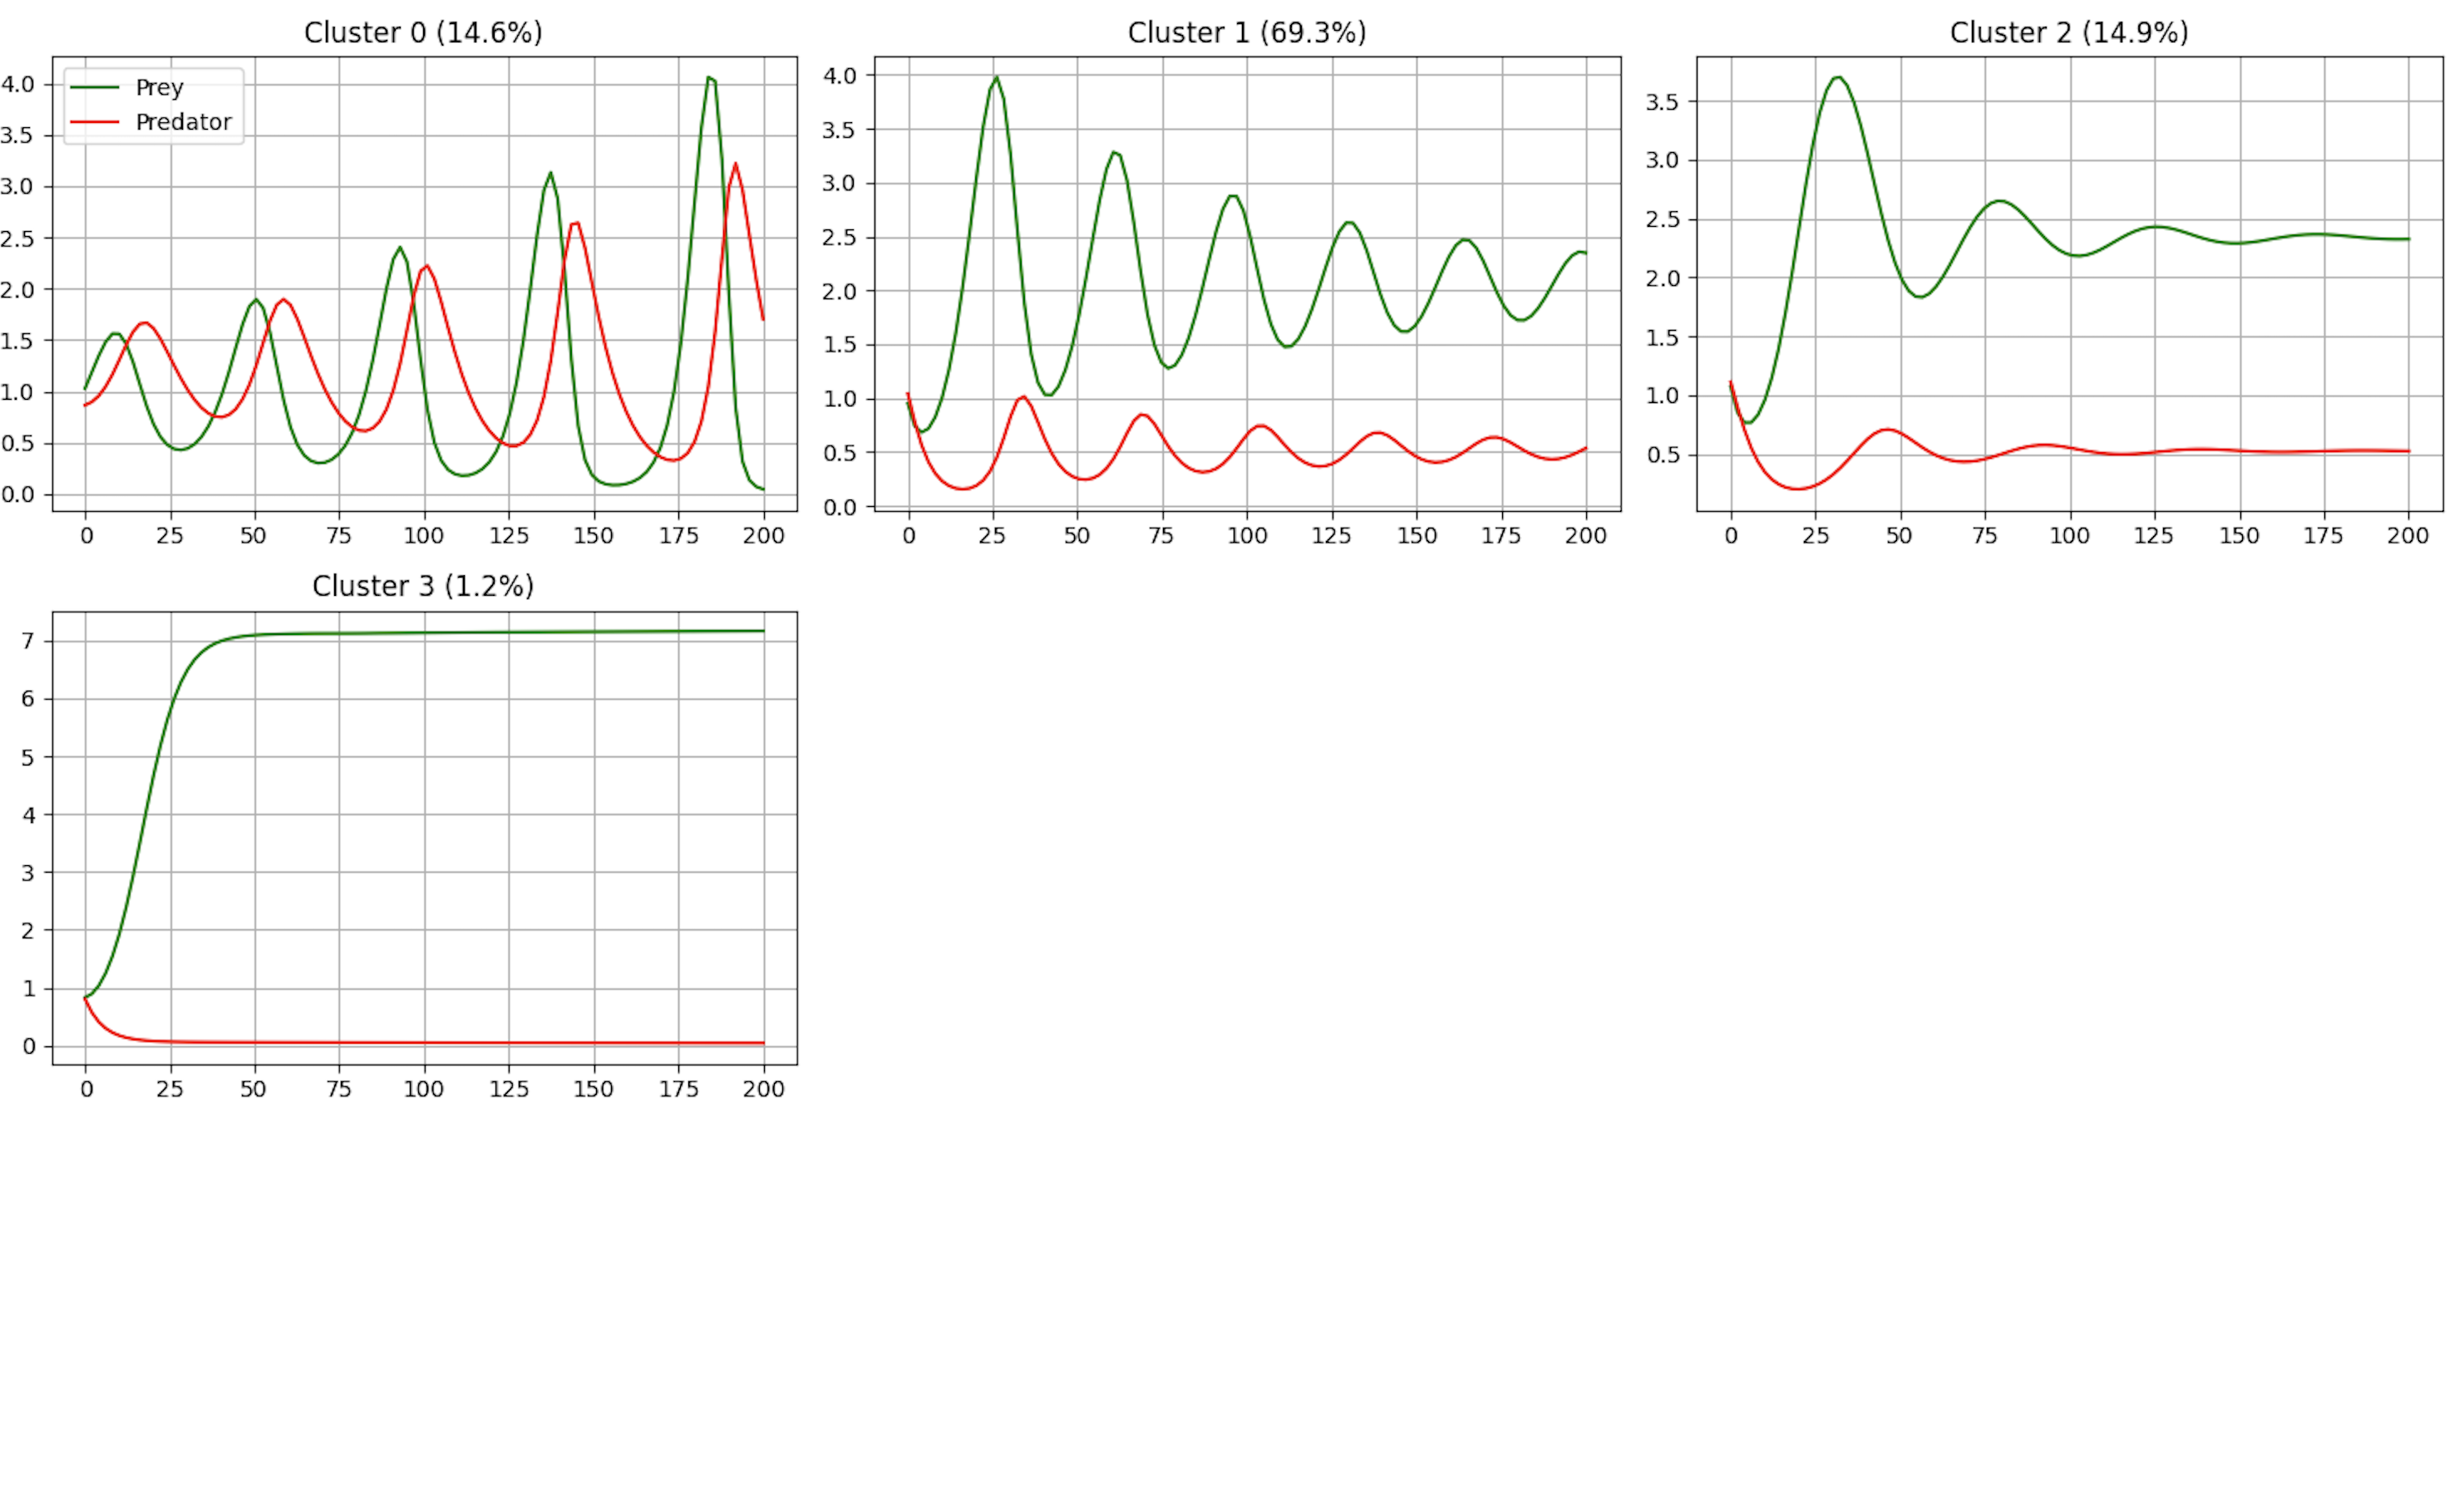
\includegraphics[width=0.8\textwidth]{cluster_representatives}
    \caption{\textbf{Cluster Analysis}. Four distinct clusters identified in the Lotka-Volterra dataset through K-means clustering}
    \label{fig:clusters}
\end{figure}

The clustering revealed that the majority of systems (69.3\%) fall into prey-dominant dynamics, suggesting parameter combinations that favor prey survival across much of the parameter space explored.

Figure \ref{fig:trajectories} showcases individual trajectories representing diverse dynamic behaviors within the dataset. These examples highlight the variability in amplitudes, frequencies, and phase relationships that our forecasting model must learn to predict accurately.

Through peak detection analysis, we calculated oscillation periods for both prey and predator populations, finding average periods of approximately 20-25 time units for prey and 20-30 time units for predators, as shown in Figure \ref{fig:periods}.

Further analysis of the phase relationships between prey and predator oscillations showed that predator peaks typically lag behind prey peaks by about 0.2 time units (20\% of the cycle period), as illustrated in Figure \ref{fig:periods}. This characteristic phase difference reflects the biological reality that predator populations grow in response to increasing prey availability, then decline as prey becomes scarce.

\begin{figure}[H]
    \centering
    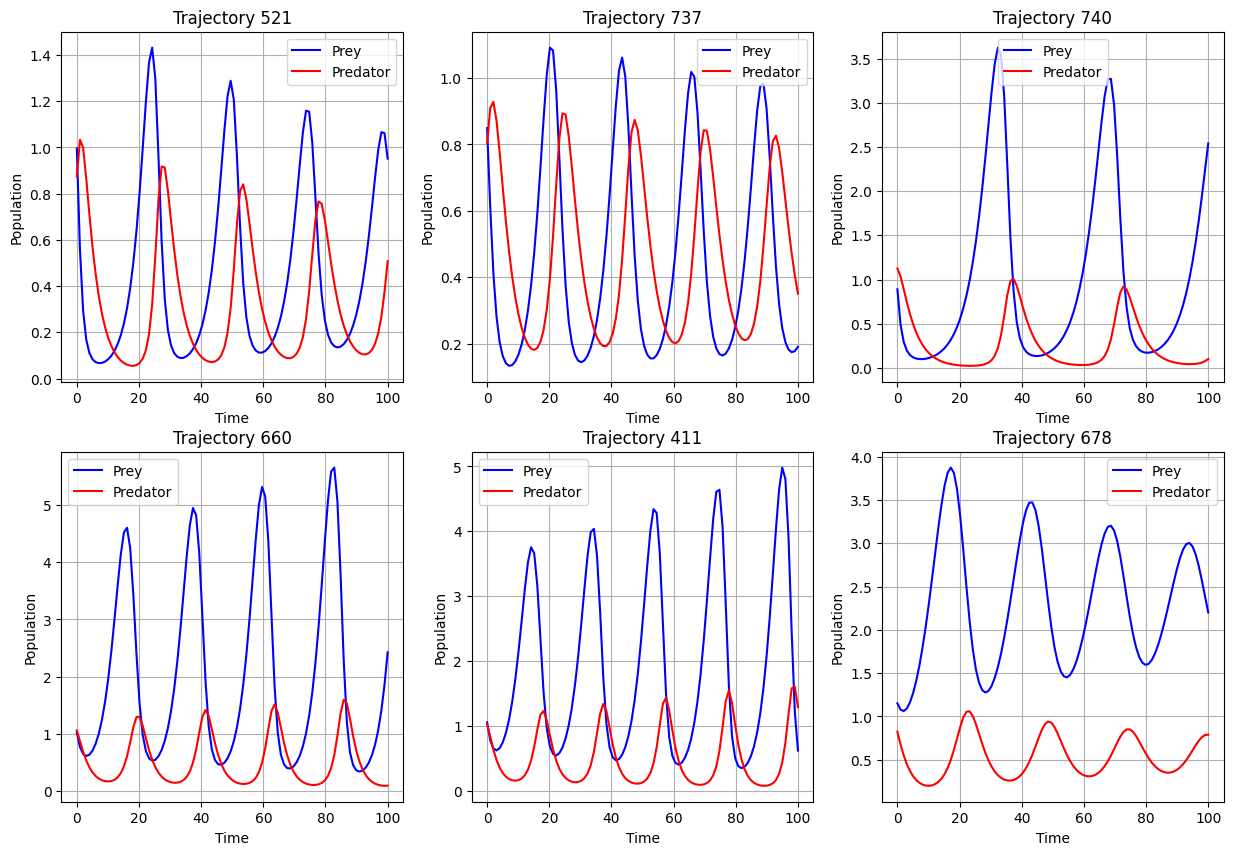
\includegraphics[width=0.8\textwidth]{sample}
    \caption{\textbf{Individual Trajectories}. Sample trajectories of prey and predator populations in the Lotka-Volterra dataset, illustrating the oscillatory dynamics characteristic of the model.}
    \label{fig:trajectories}
\end{figure}


\begin{figure} [H]
    \centering
    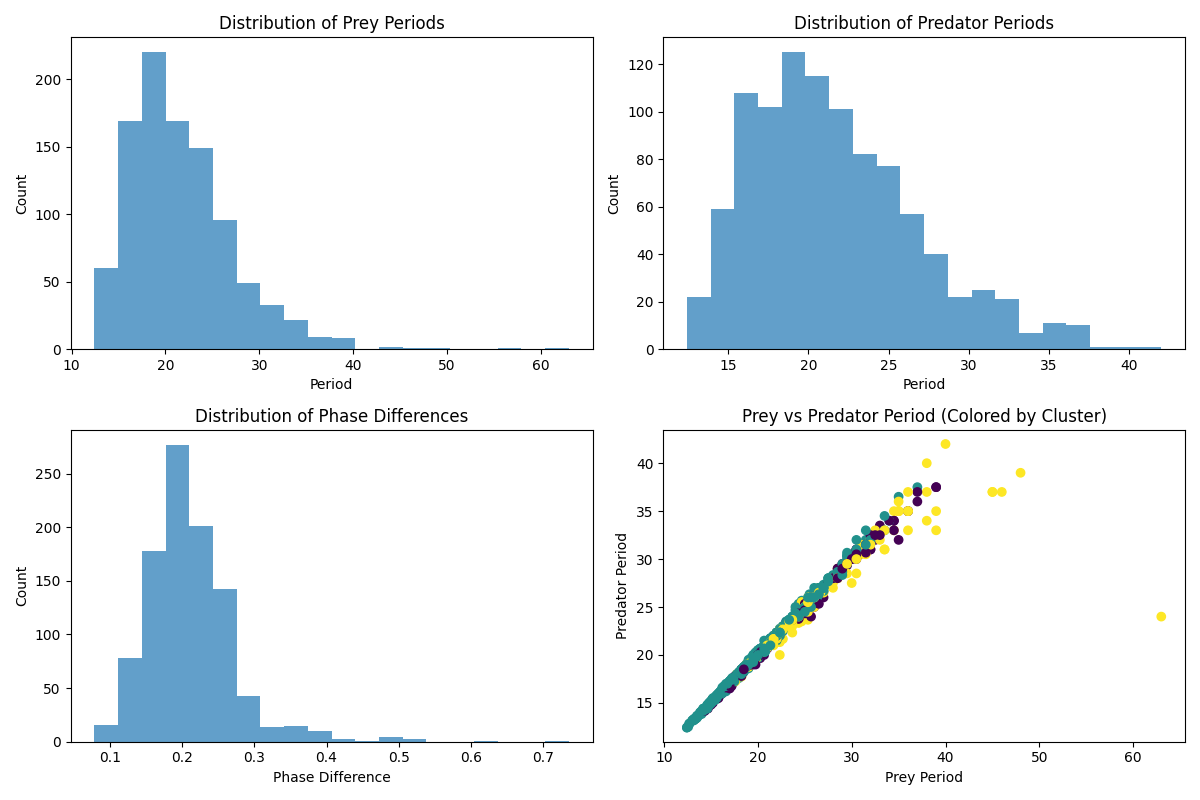
\includegraphics[width=0.8\textwidth]{period_distributions}
    \caption{\textbf{Statistical Distributions}. Distribution of oscillation periods for prey and predator populations in the Lotka-Volterra dataset, highlighting the variability in dynamics across different parameter regimes. }
    \label{fig:periods}
\end{figure}

Figure \ref{fig:average_trajectories} reveals typical system behavior with prey populations maintaining higher values (averaging $\approx$ 1.7 units) compared to predator populations (averaging $\approx$ 0.6 units) after initial transient dynamics.

\begin{figure} [H]
    \centering
    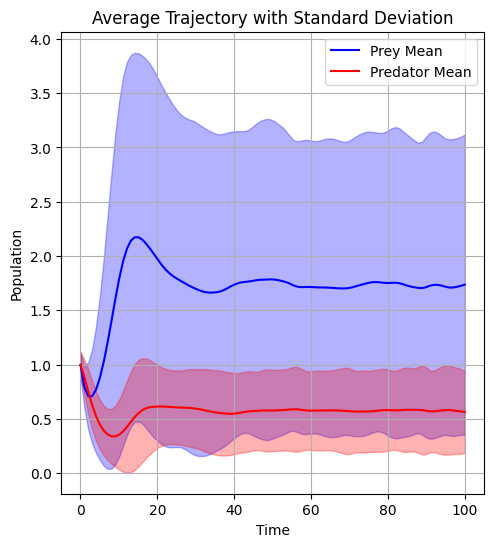
\includegraphics[width=0.5\textwidth]{overview_distribution}
    \caption{\textbf{Average Trajectories}. Average population trajectories with uncertainty: Mean prey (blue) and predator (red) population trajectories over time with shaded regions representing standard deviation.}
    \label{fig:average_trajectories}
\end{figure}

\begin{figure} [H]
    \centering
    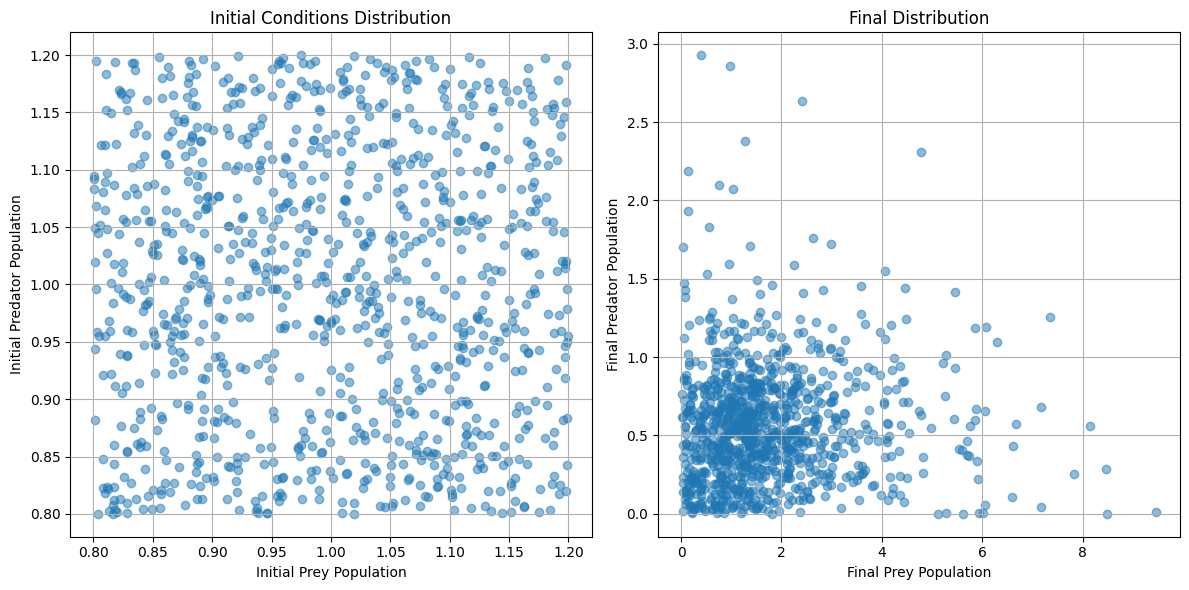
\includegraphics[width=0.8\textwidth]{initial_final_distribution}
    \caption{\textbf{Initial vs Final Distribution}. Comparison between initial conditions (left) and final states (right) of the predator-prey systems after simulation.}
    \label{fig:initial}
\end{figure}

Figure \ref{fig:initial} reveals the system's sensitivity to initial conditions, a hallmark of nonlinear dynamics. Despite starting in a narrow range (0.8-1.2 for both populations), final states diverge dramatically. The final distribution shows predator populations concentrated at lower values (0.1-1.0) while prey populations spread widely (0-8), indicating states where prey dynamics become less constrained by predator influence. This divergence highlights why long-term forecasting of such systems is challenging—small input variations amplify into significantly different outcomes over time.

For the current study with our limited dataset of 1,000 trajectories, we implemented a simple random split into training (70\%), validation (15\%), and testing (15\%) sets. Given the time constraints and dataset size, this approach provided a practical balance between model training and evaluation needs. However, the observed dynamics suggest several potential improvements for future work with larger datasets.

\subsubsection*{Future Improvements for Data Handling}
The observed sensitivity to initial conditions and the diverse range of dynamic behaviors have important implications for more sophisticated approaches to training, validation, and testing splits in future work. With a larger dataset, a stratified sampling approach based on the four identified clusters would better maintain the distribution of dynamic behaviors across all splits.

Such stratification would be particularly valuable because the complexity and diversity of the dynamics require the model to learn from examples across all behavioral regimes. For example, the rare "predator collapse" trajectories (1.2\% of cases) should be proportionally represented in all splits to prevent the model from treating such cases as anomalies during evaluation. Similarly, the phase relationships and oscillation characteristics vary systematically across clusters, making it essential that the model train on and be evaluated against the full spectrum of possible dynamics.

\subsection*{LLMTIME Preprocessing Approach}

To enable language models to process numerical time series data, we implement the LLMTIME preprocessing scheme introduced by Gruver\cite{gruver2023large}. This approach transforms multidimensional time series data into structured text representations that preserve temporal patterns while exploiting the language model's textual processing capabilities.

\subsubsection*{Text Representation Format}

While the original LLMTIME approach \cite{gruver2023large} was designed for univariate time series, our Lotka-Volterra data requires representing multiple variables (prey and predator populations) across sequential timesteps. We therefore extended the LLMTIME encoding convention using a structured delimiter system:

\begin{itemize}
    \item Comma (“,") separates different variables at the same timestep
    \item Semicolon (“;") separates different timesteps in the sequence
\end{itemize}

Our implementation supports different numerical precision formats. Below are examples showing the same trajectory segment at 3-decimal and 2-decimal precision:

\begin{verbatim}
    2.458,10.249;1.916,7.677;1.503,5.985;...  # 3-decimal precision
    2.46,10.25;1.92,7.68;1.50,5.99;...        # 2-decimal precision
\end{verbatim}



\subsubsection*{Numerical Precision Considerations}

A critical aspect of our preprocessing is determining the appropriate precision for numerical values. We implemented and tested both 2 and 3 decimal place precision options:

\begin{equation}
x_{\text{text}} = \text{round}(x, d)
\end{equation}

where $d \in \{2,3\}$ is the decimal precision. Higher precision provides more accurate population values but increases token consumption and potentially makes patterns more difficult for the model to recognize. Our hyperparameter search included precision as an experimental variable to determine its impact on forecasting performance.

\subsubsection*{Data Scaling}

To ensure numerical stability and help the model work with a consistent range of values, we apply trajectory-specific scaling to the raw data before text conversion:

\begin{equation}
x_{\text{scaled}} = x \cdot \frac{\alpha}{P_{99}(x)}
\end{equation}

where $P_{99}(x)$ is the 99th percentile of the specific time series being processed and $\alpha=10.0$ is our target scale. This approach creates a unique scaling factor for each trajectory, ensuring that most values fall within the range $[0, \alpha]$ while preserving the relative dynamics and outliers within each sequence. By computing $P_{99}$ independently for each time series, we normalize across trajectories with different magnitudes while maintaining their characteristic oscillatory patterns.

Our analysis showed that with $\alpha=10.0$, only 1\% of values exceed this threshold. This trajectory-specific scaling approach creates a more balanced distribution for the model to learn from while preserving the distinctive features of each predator-prey system.
\begin{table}[H]
    \centering
    \begin{tabular}{lc}
    \hline
    \textbf{Statistic} & \textbf{Value ($\alpha = 10.0$)} \\
    \hline
    Token Shape & [1201] \\
    Minimum Value & 1.52 \\
    Maximum Value & 10.29 \\
    Mean & 5.15 \\
    Median & 4.95 \\
    99th Percentile & 10.00 \\
    95th Percentile & 8.42 \\
    Values $>$ 10.0 & 1.0\% \\
    Values $>$ 20.0 & 0.0\% \\
    \hline
    \end{tabular}
    \caption{Statistical properties of scaled trajectory data with $\alpha = 10.0$. Note how the 99th percentile matches the target scaling value, and only 1\% of values exceed this threshold.}
    \label{tab:scaling_stats}
    \end{table}

\subsubsection*{Tokenization Effects}

The choice of text representation significantly impacts how the time series data is tokenized. For the Qwen2.5 tokenizer, numerical values are typically split into multiple tokens (e.g., 1.23 might tokenize as [1, ., 23]). Our analysis showed that each time step requires approximately 10-12 tokens, meaning that with a context length of 512 tokens, we can include roughly 40-50 time steps in the input context.

This tokenization behavior directly influenced our experimental design, particularly for evaluating optimal context length. By measuring the relationship between context length and prediction accuracy, we could determine how much historical information the model requires to make accurate forecasts.

\begin{table}[H]
\centering
\begin{tabular}{cp{3cm}cp{6cm}}
\hline
\textbf{Precision} & \textbf{Text} & \textbf{Token Count} & \textbf{Complete Token Sequence} \\
\hline
\multirow{2}{*}{2 decimal} & 10.02,10.03;7.81,7.51 & 21 & [16, 15, 13, 15, 17, 11, 16, 15, 13, 15, 18, 26, 22, 13, 23, 16, 11, 22, 13, 20, 16] \\
\cline{2-4}
    & 9.01,10.02;10.01,8.19 & 21 & [24, 13, 15, 16, 11, 16, 15, 13, 15, 17, 26, 16, 15, 13, 15, 16, 11, 23, 13, 16, 24] \\
\hline
\multirow{2}{*}{3 decimal} & 9.015,10.018;10.010,8.189 & 25 & [24, 13, 15, 16, 20, 11, 16, 15, 13, 15, 16, 23, 26, 16, 15, 13, 15, 16, 15, 11, 23, 13, 16, 23, 24] \\
\cline{2-4}
    & 10.022,10.025;7.813,7.510 & 25 & [16, 15, 13, 15, 17, 17, 11, 16, 15, 13, 15, 17, 20, 26, 22, 13, 23, 16, 18, 11, 22, 13, 20, 16, 15] \\
\hline
\end{tabular}
\caption{Complete tokenization comparison between 2-decimal and 3-decimal precision formats for predator-prey data. Note that 3-decimal precision requires approximately 19\% more tokens (25 vs 21) for representing the same underlying information. The individual tokens show how numbers, decimal points, and delimiters are broken down by the tokenizer.}
\label{tab:precision_comparison}
\end{table}
\subsubsection*{Text-to-Numeric Conversion}

To convert the model's text output back into numerical values, we implemented a simple parsing function that reverses the tokenization process. This function takes the generated text and splits it based on the defined delimiters (commas and semicolons) to reconstruct the original numerical values. The conversion process also includes scaling back to the original range using the inverse of the scaling factor applied during preprocessing.

To handle potential generation errors, the implementation employs regex pattern matching to identify numerical values despite formatting inconsistencies, gracefully processes missing or malformed values, validates physical plausibility (enforcing non-negativity for population data), and verifies dimensional consistency between predictions and targets. These safeguards ensure that evaluation metrics reflect genuine forecasting errors rather than parsing artifacts, providing a fair assessment of the model's predictive capabilities.
\subsubsection*{Training Data Processing}

For model training, we processed the data as follows:
\begin{enumerate}
    \item Split the 1,000 trajectories into train (70\%), validation (15\%), and test (15\%) sets
    \item Convert numerical trajectories to text format with specified precision and scaling
    \item For training data, create overlapping chunks with sequence length 512 and stride 256
    \item For validation, create non-overlapping chunks to prevent information leakage
    \item For testing, maintain complete trajectories without chunking
\end{enumerate}

The chunking strategy helps to maximize the utility of training data while ensuring the model sees diverse sections of trajectories during training. The stride of 256 tokens provides a 50\% overlap between consecutive chunks, helping the model learn to generate consistent predictions across different context windows.

\subsection*{FLOPs Calculation}

To rigorously assess computational efficiency, we implemented a detailed floating-point operations (FLOPs) tracking mechanism for both training and inference. This approach provides a hardware-independent measure of computational cost, enabling fair comparison across different model configurations. During calculation, we ignore the effet of grouped query attention (GQA) and KV caching on FLOP counts, as these optimizations are not directly relevant to the core operations of the model. We also exclude the impact of tokenization and text-to-numeric conversion, as these processes are not part of the model's architecture.

For the standard transformer operations, we account for all major computational components:

\begin{itemize}
    \item \textbf{Embedding layer}: Token embedding and positional encoding (RoPE)
    \item \textbf{Attention mechanism}: Query, key, value projections, attention score computation, softmax operations, and output projections
    \item \textbf{Feed-forward networks}: Gate projections, up projections, SwiGLU activations, and down projections
    \item \textbf{Normalization layers}: RMSNorm operations across all transformer layers
    \item \textbf{Language model head}: Matrix multiplication between hidden states and vocabulary embeddings
\end{itemize}

With LoRA, we modify weight matrices using low-rank decomposition: $W = W_0 + BA$ where $B \in \mathbb{R}^{d \times r}$ and $A \in \mathbb{R}^{r \times k}$ with rank $r \ll \min(d,k)$. The FLOPs for each LoRA-augmented projection are:

\begin{align}
\text{FLOPs}_{\text{LoRA}} &= \text{FLOPs}_{\text{original}} + \text{FLOPs}_{x \times A^T} + \text{FLOPs}_{(xA^T) \times B^T}\\
&= BS \cdot H \cdot (2H - 1) + BS \cdot r \cdot (2H - 1) + BS \cdot H \cdot (2r - 1)
\end{align}

where $B$ is batch size, $S$ is sequence length, $H$ is hidden dimension, and $r=8$ is the LoRA rank.

The total training FLOPs include both forward and backward passes. For the backward pass, we use the standard approximation of doubling the forward pass FLOPs, resulting in a 3× multiplier for training steps (1× forward + 2× backward).

We established a total computational budget of $10^{17}$ FLOPs for our experiments, carefully tracking usage throughout the development process. This budget was allocated across hyperparameter search (50\%), context length evaluation (15\%), and final training (35\%). A full breakdown of FLOP calculations for all operations is provided in the Appendix.

\section*{Implementation}

\subsection*{Hardware}
All experiments were conducted on NVIDIA A100 GPU instances with 40GB of RAM. All inferences of models were performed on Mac M1 Pro Chip with 16GB of RAM. 
Our implementation includes fallback mechanisms for different hardware accelerators, automatically selecting the optimal device (CUDA, MPS, or CPU) based on availability.

\subsection*{Model training setup}
\subsubsection*{Optimization Approach}

We employed the AdamW optimizer with weight decay of 0.01, which helps mitigate overfitting during fine-tuning. Gradient clipping at 1.0 was applied to prevent exploding gradients, which is particularly important when fine-tuning large language models. For each training step, we logged both pre-clipping and post-clipping gradient norms, maintaining a ratio typically between 0.8-1.0, indicating stable training dynamics.

\begin{figure}[h]
    \centering
    \begin{minipage}{0.48\textwidth}
        \centering
        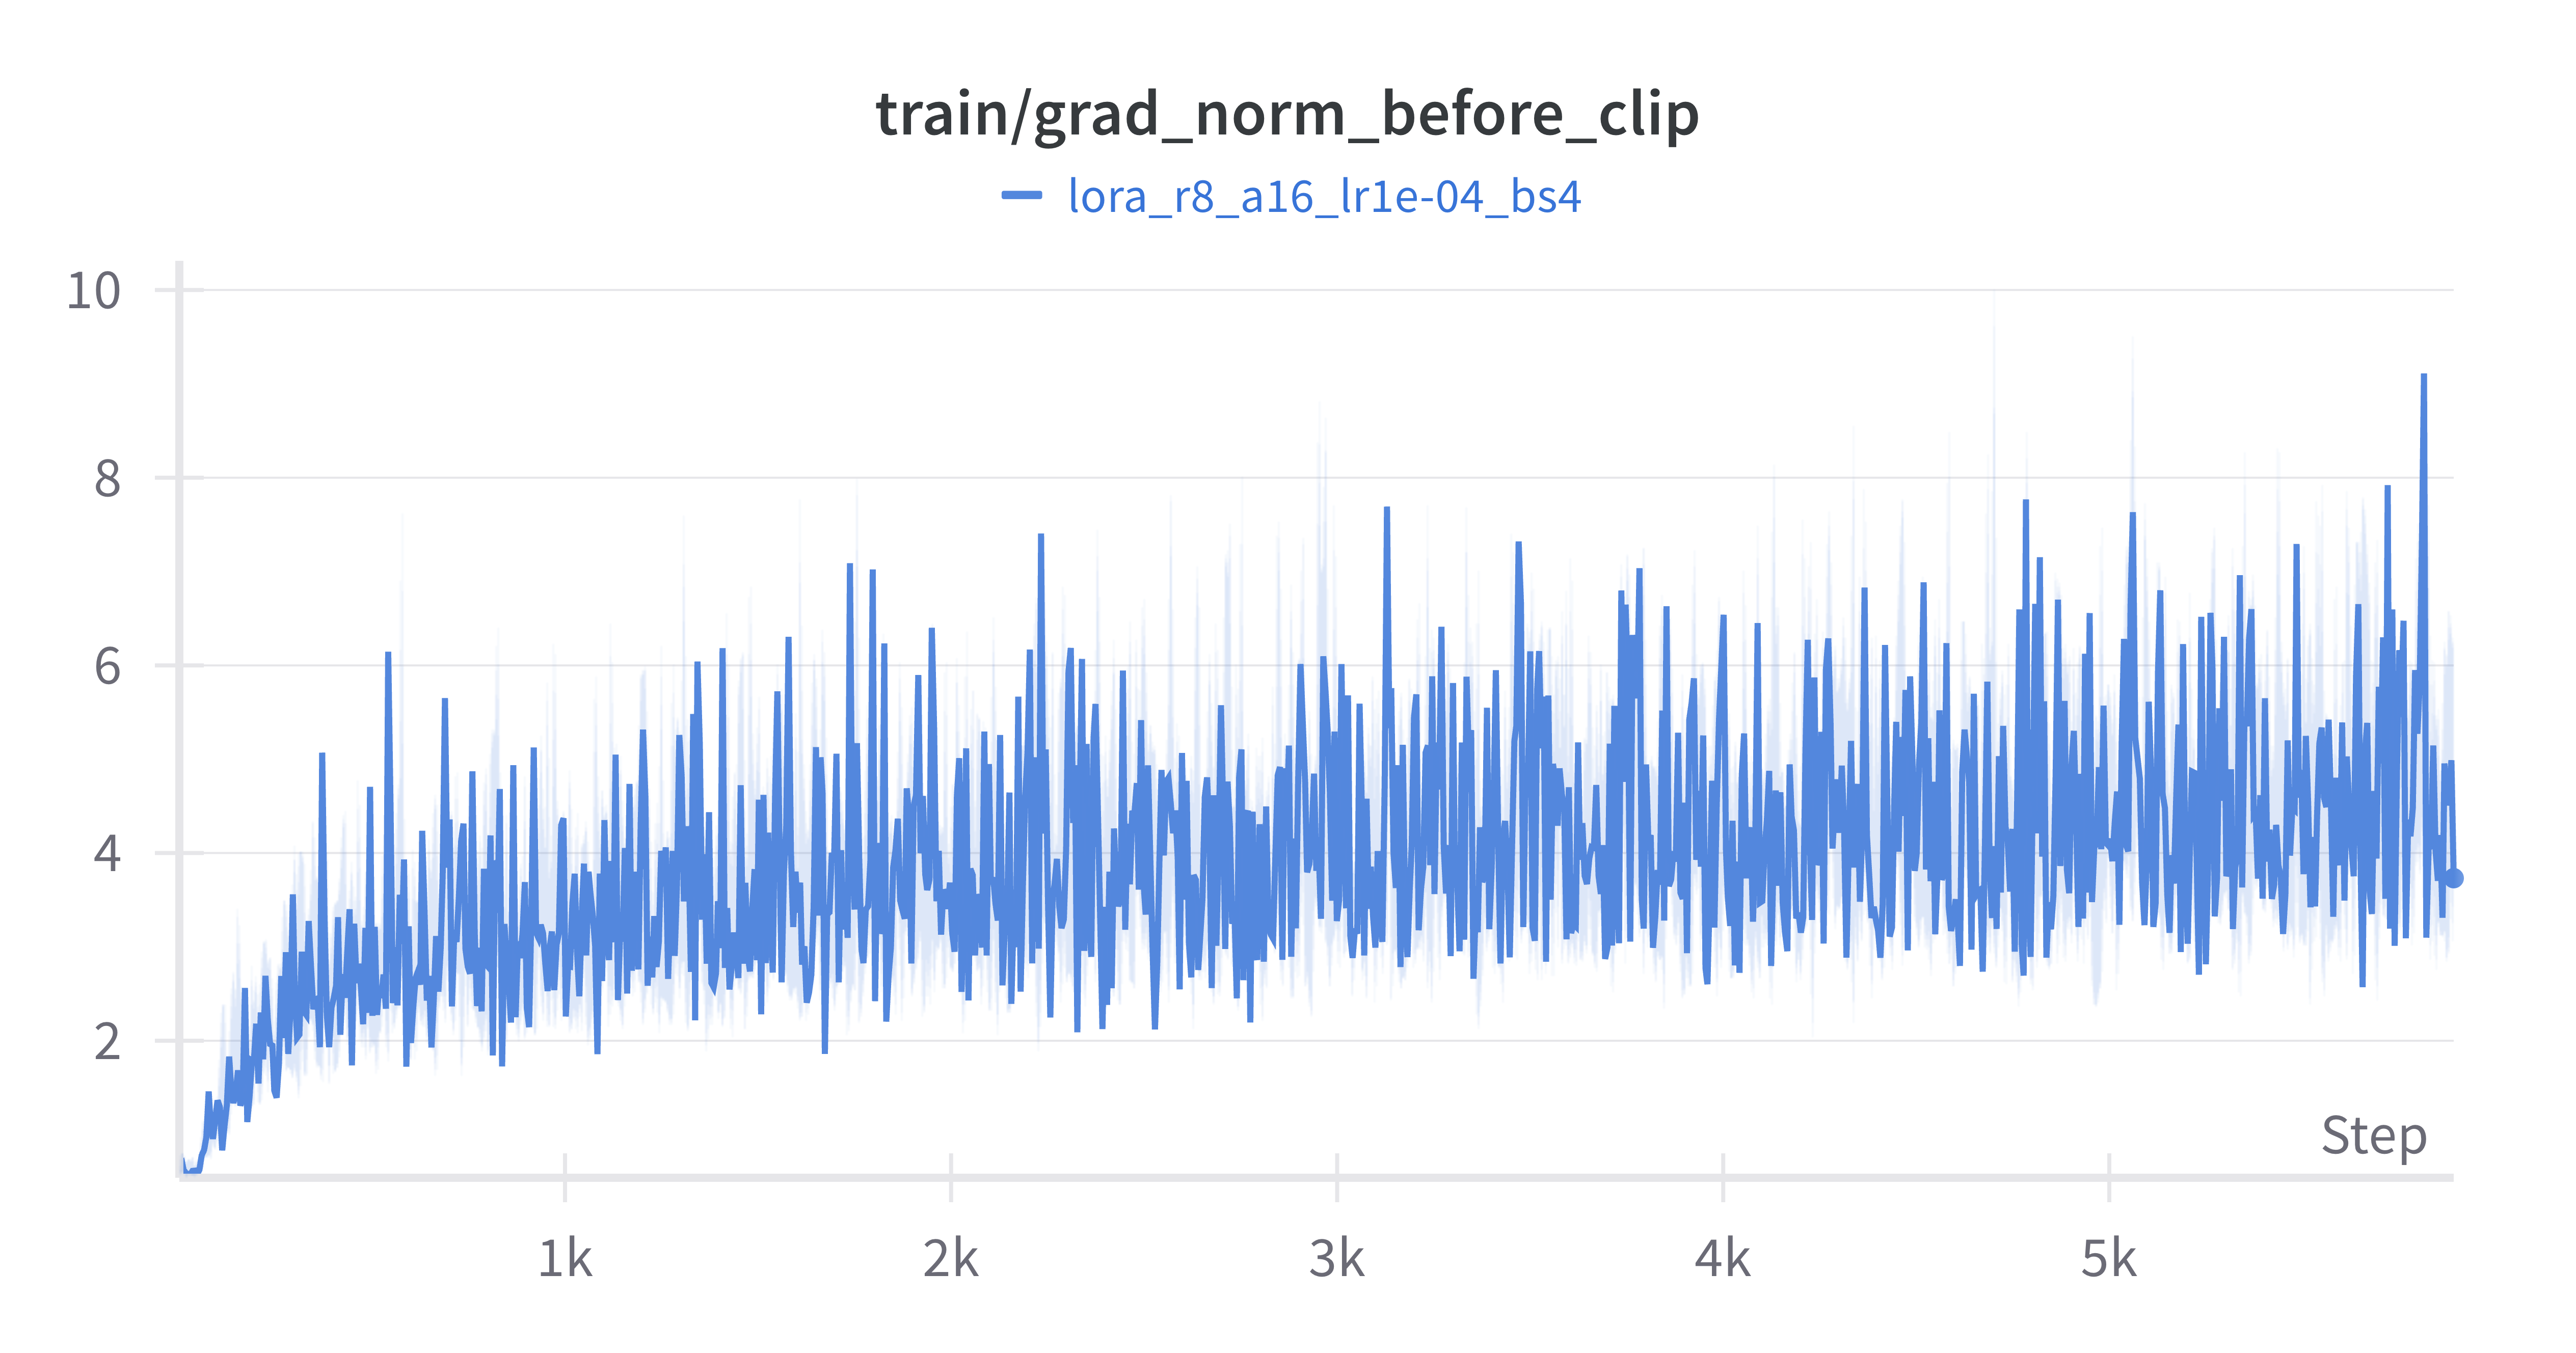
\includegraphics[width=\textwidth]{before}
        \label{fig:first_label}
    \end{minipage}
    \hfill
    \begin{minipage}{0.48\textwidth}
        \centering
        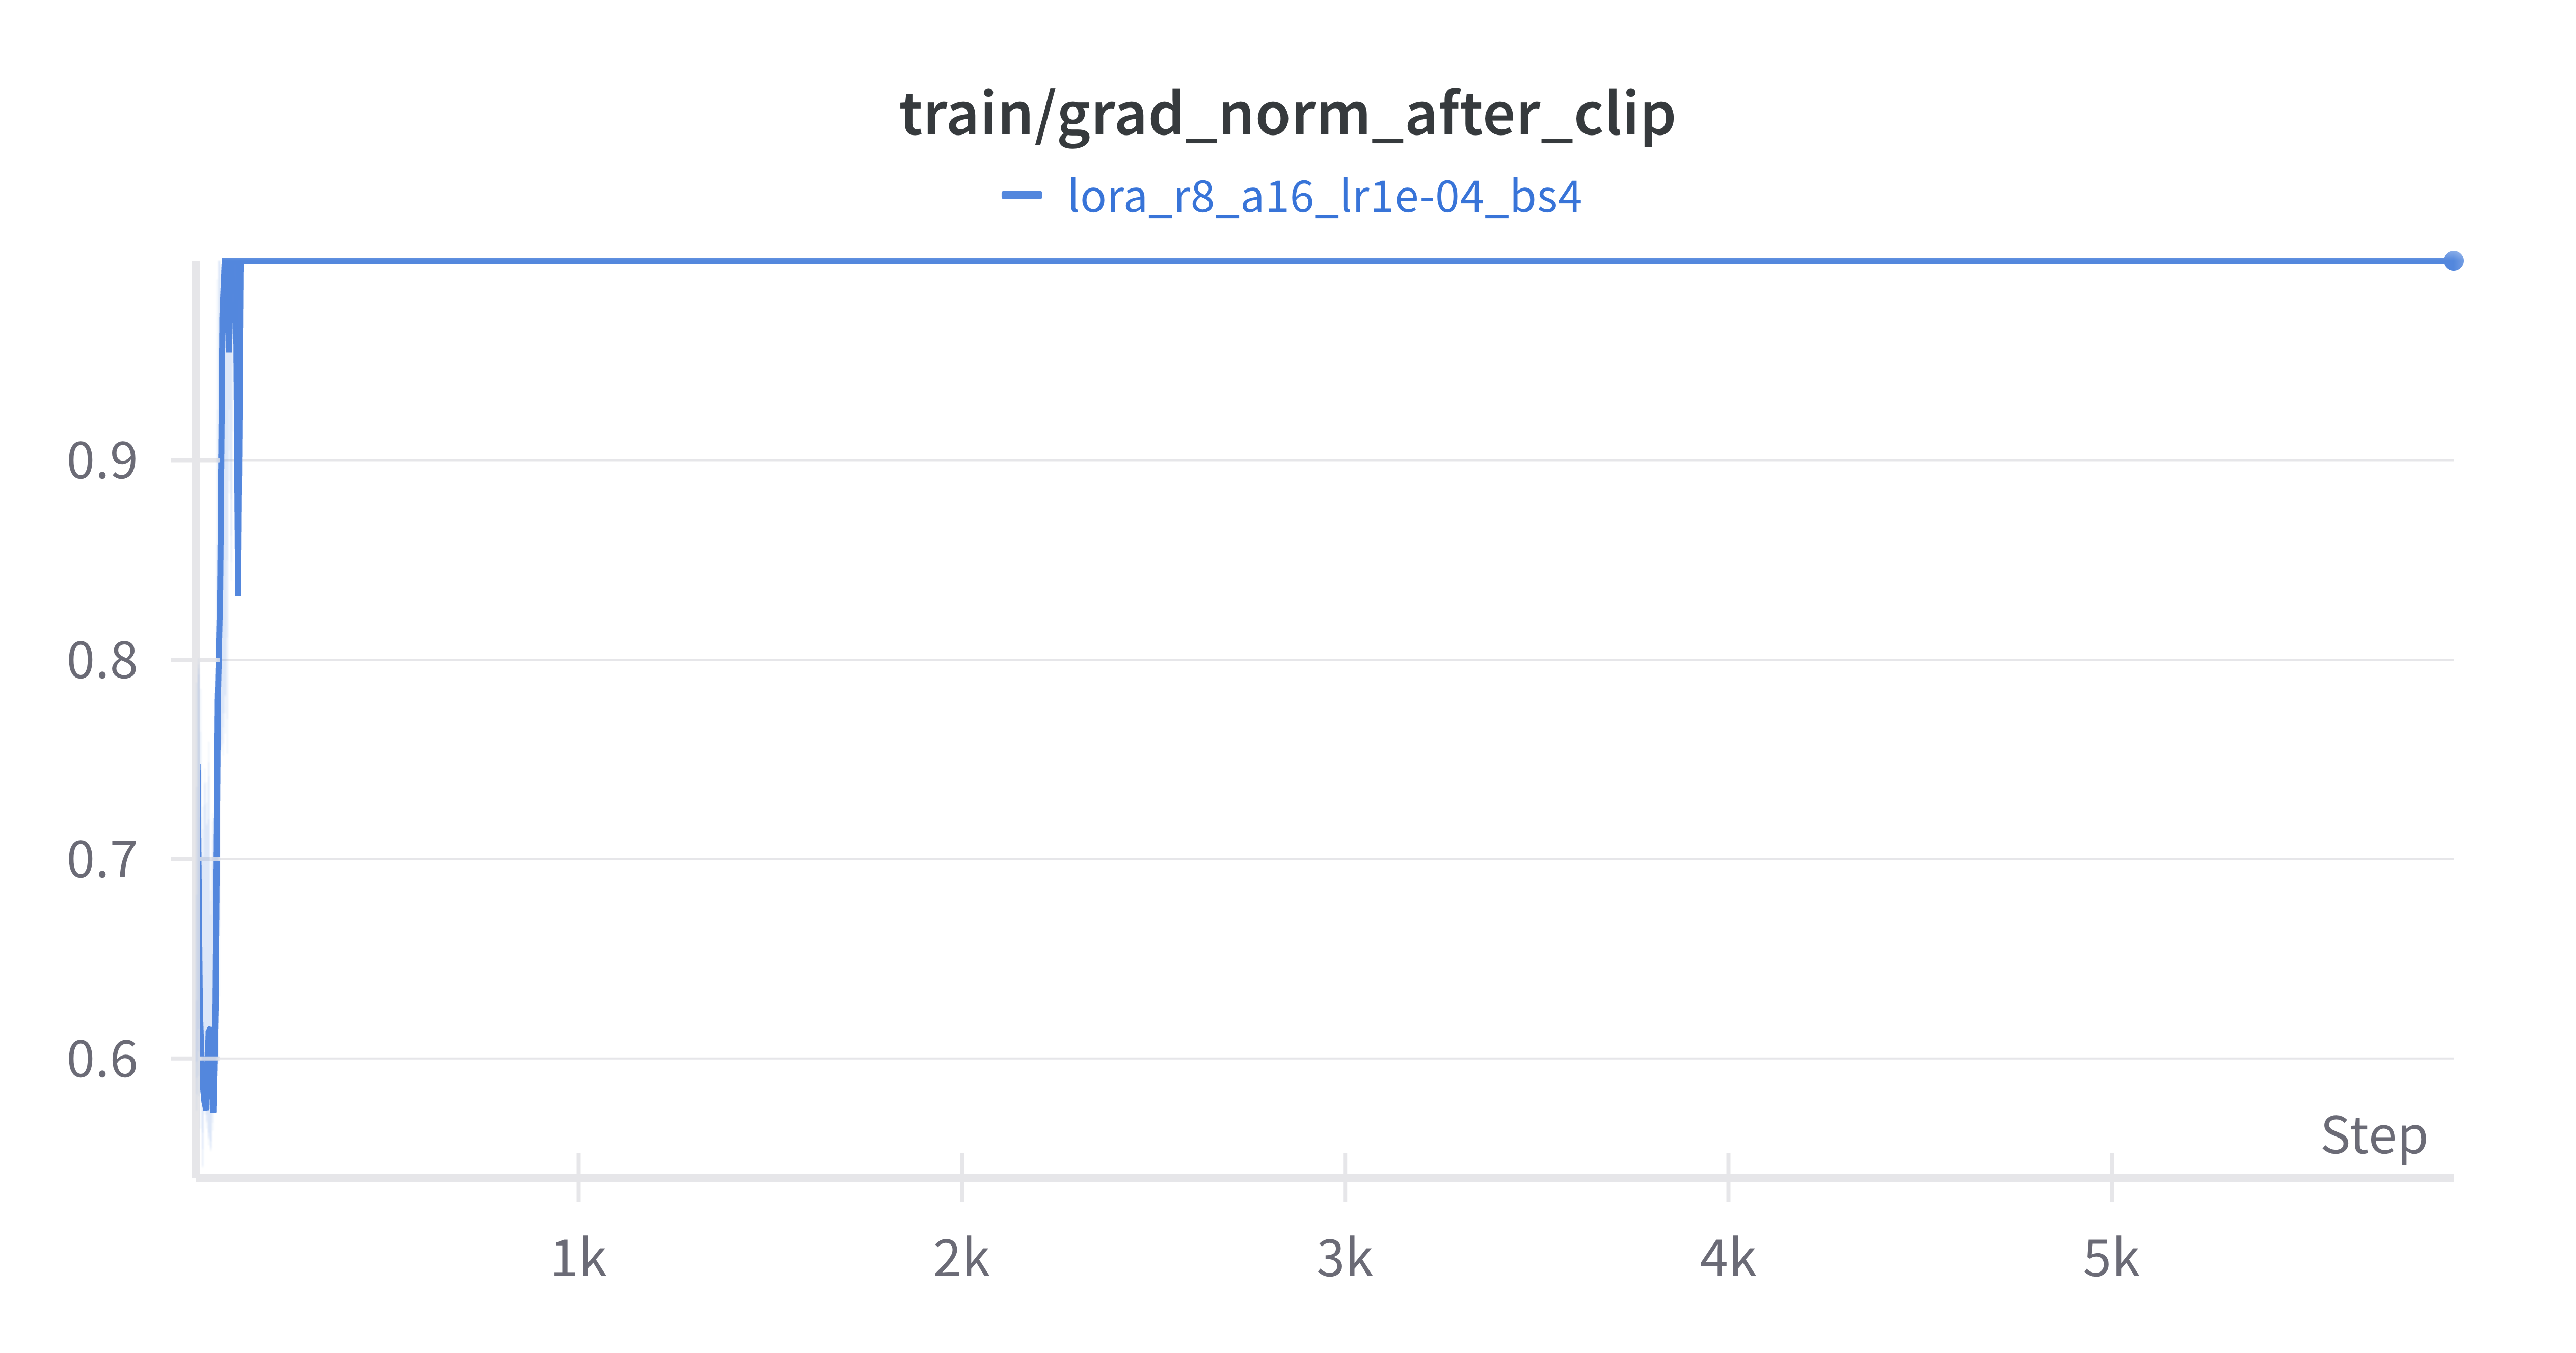
\includegraphics[width=\textwidth]{after}
        \label{fig:second_label}
    \end{minipage}
    \caption{\textbf{Gradient norm comparison} Left: The plot shows increasing gradient magnitudes as training progresses, with values ranging from approximately 1 to 9. Right: The values are consistently maintained at or below 1.0 throughout training, demonstrating the effectiveness of gradient clipping.}
\end{figure}
We utilized the OneCycleLR scheduler which provides effective learning rate management through three phases:
\begin{itemize}
    \item A warm-up phase (10\% of total steps) where learning rate gradually increases
    \item  A sustained high-learning-rate phase
    \item  A cool-down phase with annealed learning rates   
\end{itemize}
This approach allows the model to initially adapt quickly and then gradually refine its parameters.

\subsubsection*{Validation Set up}
The validation step is an inference-based process that evaluates the model's performance on unseen data. We implemented a validation loop that runs every 500 steps during training, allowing us to monitor the model's performance. We used 30 samples from validation with random seed, perfomed mae and mse when predicting three time steps ahead. The validation set is used to track the model's performance and prevent overfitting. We also implemented a checkpointing mechanism to save the best-performing model based on validation metrics. 


\subsection*{Evaluation Setup}
Our evaluation pipeline implements a rigorous approach for assessing forecasting accuracy:
\subsubsection*{Forecasting Process}

For each test trajectory, we:
\begin{enumerate}
    \item Provide the first 50 timesteps as context
    \item Generate the next 50 timesteps autoregressively
    \item Apply post-processing to ensure valid numerical formatting
    \item Compare predictions against ground truth values
\end{enumerate}

To ensure robustness, we implemented pattern-matching techniques that correct common errors in the model's text generation, such as inconsistent decimal places or missing delimiters.

\subsubsection*{Evaluation Metrics}

We calculated the following metrics to assess model performance:

\begin{itemize}
    \item \textbf{Mean Absolute Error (MAE)}: Primary metric for overall accuracy assessment, measuring absolute difference between predicted and actual values.
    \item \textbf{Mean Squared Error (MSE)}: Secondary metric that penalizes larger errors more heavily. 
    \item \textbf{Population-specific metrics}: Separate MAE and MSE values for prey and predator populations, capturing the model's ability to forecast different variables.
    \item \textbf{Success rate}: Percentage of trajectories where the model generated valid numerical predictions that could be parsed correctly.
\end{itemize}

Each test run involved evaluating 150 trajectories, with detailed performance tracking for both population variables across all generated timesteps.
\subsubsection*{Generation Settings}

For model generation, we followed the same approach as the original LLMTIME paper \cite{gruver2023large}, using stochastic sampling with temperature 0.9 and top-p 0.9:

\begin{verbatim}
output = model.generate(
    inputs["input_ids"],
    max_new_tokens=max_tokens,
    temperature=0.9,
    top_p=0.9,
    do_sample=True,
    renormalize_logits=True
)
\end{verbatim}

This configuration provides a balance between diversity and coherence in generated sequences, which is particularly important for producing accurate numerical forecasts while maintaining the ability to capture the range of possible system behaviors.
\section*{LoRA Experiments}
\subsection*{Hyperparameter search experiment}
To optimize our LoRA fine-tuning approach, we conducted a comprehensive grid search over key hyperparameters, evaluating their impact on forecasting accuracy while respecting our computational budget constraints.


\subsection*{Context Length Exploration}
\subsection*{Analysis of results}

\section*{Model Performance Comparison}

\begin{itemize}
    \item Detailed analysis of the best model configuration
   \item  Comparative evaluation against baseline
   \item  Visualization of forecasting performance
   \item Error analysis for prey and predator populations
\end{itemize}

\section*{ Discussion}
\begin{itemize}
    \item Analysis of the trade-offs between computational cost and accuracy
\item Impact of different hyperparameters on performance
\item Strengths and limitations of the approach
\item Recommendations for time-series fine-tuning under tight compute budgets
\end{itemize}


\section*{Conclusion}

\begin{itemize}
    \item  Summary of key findings
     \item Suggestions for future improvements
     \item Final FLOP accounting table
\end{itemize}

\section*{Appendix}
\subsection*{Detailed FLOP Calculation}

This section provides a comprehensive accounting of the floating-point operations (FLOPs) used in our experiments with the Qwen2.5-0.5B model, based on our custom FLOP tracking implementation.

\subsubsection*{Forward Pass Components}

For a single forward pass with sequence length $S$, batch size $B$, hidden dimension $H=896$, intermediate dimension $I=4864$, and vocabulary size $V=151,936$, we calculate FLOPs for each component as follows:

\paragraph{Embedding Layer}
The token embedding lookup is primarily a memory operation rather than computational, counted as:
\begin{equation}
\text{FLOPs}_{\text{embedding}} = B \times S \times H = 64 \times 512 \times 896 \approx 2.94 \times 10^7 \text{ FLOPs}
\end{equation}

\paragraph{Attention Mechanism with LoRA}
For each attention layer:
\begin{enumerate}
    \item \textbf{Query projection with LoRA}: For modules with LoRA enabled (rank $r=8$):
    \begin{align}
    \text{FLOPs}_{\text{q\_proj}} &= \text{FLOPs}_{\text{original}} + \text{FLOPs}_{x \times A^T} + \text{FLOPs}_{(xA^T) \times B^T}\\
    &= B\times S \times H \times (2H-1) \\
    &+ B\times S \times r \times (2H-1) + B\times S \times H \times (2r-1)
    \end{align}
    
    \item \textbf{Key/Value projections}: Similar to query.
    \item \textbf{RoPE}: $B\times S \times 3 \times \text{num\_heads} \times \text{head\_dim} + 0.5 \times B \times S \times \text{num\_heads} \times \text{head\_dim}$, here we only negate half of the original length of x.
    \item \textbf{Attention scores}: $B\times S \times \text{num\_heads} \times S \times (2 \times \text{head\_dim} - 1)$
    \item \textbf{Attention mask}: $B \times \text{num\_heads} \times S \times S$
    \item \textbf{Attention softmax}: $B \times \text{num\_heads} \times S \times (12S - 1)$
    \item \textbf{Weighted sum}: $B \times \text{num\_heads} \times S \times \text{head\_dim} \times (2S - 1)$
    \item \textbf{Output projection}: Similar structure to query projection if LoRA is applied
\end{enumerate}

\paragraph{Feed-Forward Network}
\begin{enumerate}
    \item \textbf{Gate and Up projections}: $2 \times B\times S \times I \times (2H - 1)$
    \item \textbf{SwiGLU activation}: $B\times S \times I \times 14$
    \item \textbf{Element-wise multiplication}: $B\times S \times I$
    \item \textbf{Down projection}: $B\times S \times H \times (2I - 1)$
\end{enumerate}

\paragraph{Layer Normalization and Residuals}
\begin{enumerate}
    \item \textbf{RMSNorm (2 per layer)}: $2 \times B\times S \times (4H + 12)$
    \item \textbf{Residual connections}: $2 \times B\times S \times H$
\end{enumerate}

\paragraph{Output Layer}
\begin{enumerate}
    \item \textbf{Final RMSNorm}: $ B \times S (4 \times H+12) FLOPs$
    \item \textbf{LM head}: $2 \times B \times S \times H \times V = 2 \times B \times S \times 896 \times 151936$ FLOPs
\end{enumerate}

\subsubsection*{Total Forward Pass FLOPs}

For our configuration with $H=896$, $I=4864$, and 24 layers, the total forward pass FLOPs for batch size $B=4$ and sequence length $S=512$ is approximately:
\begin{align}
\text{FLOPs}_{\text{forward}} \approx & 1.98 \times 10^{12} \text{ FLOPs} 
\end{align}

\subsubsection*{Training Step FLOPs}

For training, our implementation uses the standard approximation that backward pass requires twice the computation of the forward pass (in the same setting as in forward pass):
\begin{equation}
\text{FLOPs}_{\text{training\_step}} = \text{FLOPs}_{\text{forward}} + 2 \times \text{FLOPs}_{\text{forward}} \approx 5.94 \times 10^{12} \text{ FLOPs}
\end{equation}

\subsubsection*{Budget Allocation and Usage}

Our implementation tracked FLOPs throughout the experimental process, including:
\begin{table}[h]
    \centering
    \begin{tabular}{lcc}
    \hline
    \textbf{Experiment} & \textbf{Total FLOPs} & \textbf{Budget Percentage} \\
    \hline
    \multicolumn{3}{c}{\textbf{Hyperparameter Grid Search (18 configurations)}} \\
    \hline
    Average per Hyperparameter Config & 2.70$\times$ 10$^{15}$ & 2.7\% \\
    Total Grid Search (18 Experiments) & 4.86 $\times$ 10$^{16}$ & 48.6\% \\
    \hline
    \multicolumn{3}{c}{\textbf{Context Length Evaluation}} \\
    \hline
    Context Length 768 & 9.10 $\times$ 10$^{15}$ & 9.1\% \\
    Context Length 512 & 5.94$\times$ 10$^{15}$ & 5.9\% \\
    Context Length 128 & 1.43 $\times$ 10$^{15}$ & 1.4\% \\
    \hline
    \multicolumn{3}{c}{\textbf{Final Fine-tuning (LoRA)}} \\
    \hline
    LoRA (r=8, $\alpha$=16, lr=1e-04, bs=4) & 3.50 $\times$ 10$^{16}$ & 35\% \\
    \hline
    \multicolumn{3}{c}{\textbf{Overall FLOP Usage}} \\
    \hline
    Total Experimental FLOPs & 1.0 $\times$ 10$^{17}$ & 100.0\% \\
    Maximum Budget & 1.0 $\times$ 10$^{17}$ & 100.0\% \\
    \hline
    \end{tabular}
    \caption{FLOPs Usage Across Experiments}
    \label{tab:flops_usage}
    \end{table}
    

\bibliographystyle{plain}
\bibliography{references}
\end{document}